\documentclass[conference]{IEEEtran}
\IEEEoverridecommandlockouts

% ── Packages ─────────────────────────────────────────────────────────────────
\usepackage{cite}
\usepackage{amsmath,amssymb}
\usepackage{graphicx}
\usepackage{booktabs}
\usepackage{multirow}
\usepackage{array}
\usepackage{url}
\usepackage{xcolor}
\usepackage{tikz}
\usetikzlibrary{arrows.meta,positioning,shapes.geometric}
\usepackage{stfloats}
\usepackage{placeins}   % \FloatBarrier
\usepackage{tabularx}
\newcolumntype{J}[1]{>{\raggedright\arraybackslash}p{#1}}
\newcolumntype{K}{>{\raggedright\arraybackslash}X}

% ── Title & Author ────────────────────────────────────────────────────────────
\title{Failure Injection and Propagation Analysis in Agentic Microservice
  Workflows: Evidence from Google-Bench and Retail-Bench Scenarios}

\author{%
  \IEEEauthorblockN{Deepak Sunil Chavan}
  \IEEEauthorblockA{%
    Department of Electrical and Computer Engineering\\
    Concordia University, Montreal, Canada\\
    Email: deepaksunil.chavan@concordia.ca}}

% ═════════════════════════════════════════════════════════════════════════════
\begin{document}
\maketitle

% ── Abstract ─────────────────────────────────────────────────────────────────
\begin{abstract}
Agentic microservices introduce adaptive reasoning and tool orchestration,
but also new fault surfaces that are difficult to validate using conventional
microservice testing. This paper presents a controlled fault-injection study
across seven instrumented agent services in the LLM-MAS architecture and
evaluates fault reachability, infection, and propagation using
checkpoint-based tracing (LKW+RIP). We execute two benchmark suites
(Google-bench followed by Retail-bench) on an HPC environment and map observed
failures to MAST-style fault categories. Six Python-based agents serve as
deterministic framework-validation baselines (no LLM in the loop); the
ShippingService agent is the sole live-LLM service, exercised with
\texttt{qwen2.5-coder:14b} via Ollama on Concordia SPEED HPC. Across all
64~mode-runs (6 deterministic agents $\times$ 9 fault modes $\times$ 3
stability runs), zero UNSTABLE entries were observed, confirming 100\%
reproducibility of the LKW+RIP instrumentation framework. For the
ShippingService, 9 of 11 fault modes produced observable LKW signals (7 TP,
2~Partial TP, 1 TN); 1 fault mode remains INCONCLUSIVE due to LLM inference
timeout under the compliance-ambiguity scenario. Per-benchmark root cause
analysis shows that FM-2.2 (hallucinated output) is the highest-risk fault
class at both single-agent and cross-agent boundaries, completing all
checkpoints with zero propagation depth while silently corrupting downstream
state. We provide automated HITL tier classification and inter-agent
propagation evidence to identify which faults are silently absorbed, which
propagate to business-harmful states, and which require human intervention.
Key limitations are documented: the six deterministic agents validate the
instrumentation framework rather than LLM-based fault detection capability,
and the compliance-ambiguity fault mode remains unresolved at model scales
tested.
\end{abstract}

\begin{IEEEkeywords}
agentic systems, fault injection, microservices, root cause analysis,
propagation analysis, LLM reliability
\end{IEEEkeywords}

% ═════════════════════════════════════════════════════════════════════════════
\section{Introduction}
% ═════════════════════════════════════════════════════════════════════════════

Agent-driven microservices combine tool-calling, reasoning loops, and external
side effects (e.g., carrier selection, tracking generation, persistence). While
this increases autonomy, it can introduce latent failures not captured by unit
or API tests. Our goal is to evaluate whether controlled faults can be injected,
reproduced, observed, and contained before they become business harm.

This study covers seven agent services in the LLM-MAS architecture: six
Python-based agents (PaymentAgent, CurrencyAgent, EmailServiceAgent,
ProductCatalogAgent, RecommendationAgent, AdServiceAgent) that serve as
deterministic instrumentation baselines, and the ShippingService agent, which
is the sole live-LLM service using \texttt{qwen2.5-coder:14b} via Ollama on
Concordia SPEED HPC. This design separates framework validation (six agents)
from LLM-in-the-loop capability testing (ShippingService).

In this project, we answer the following research questions:
\begin{enumerate}
  \item Can realistic faults be injected into an agent-driven service and
        reliably reproduced?
  \item Where does failure first appear in the execution flow?
  \item How far does it propagate downstream?
  \item Which failures can be auto-resolved by agents, and which require human
        intervention?
  \item How stable are these observations across repeated runs in a controlled
        compute environment?
\end{enumerate}

% ═════════════════════════════════════════════════════════════════════════════
\section{System and Fault Model}
% ═════════════════════════════════════════════════════════════════════════════

\subsection{Target Workflow}
We evaluate an order orchestration flow with agentic steps:
\begin{center}
\small
\texttt{TASK\_START} $\!\to\!$ \texttt{QUOTE\_DONE} $\!\to\!$ \texttt{CARRIER\_DONE}
$\!\to\!$ \texttt{TRACKING\_DONE} $\!\to\!$ \texttt{SAVE\_DONE}
$\!\to\!$ \texttt{ESCALATION\_CHECK} $\!\to\!$ \texttt{FINAL\_ANSWER}
\end{center}

\begin{figure*}[t]
\centering
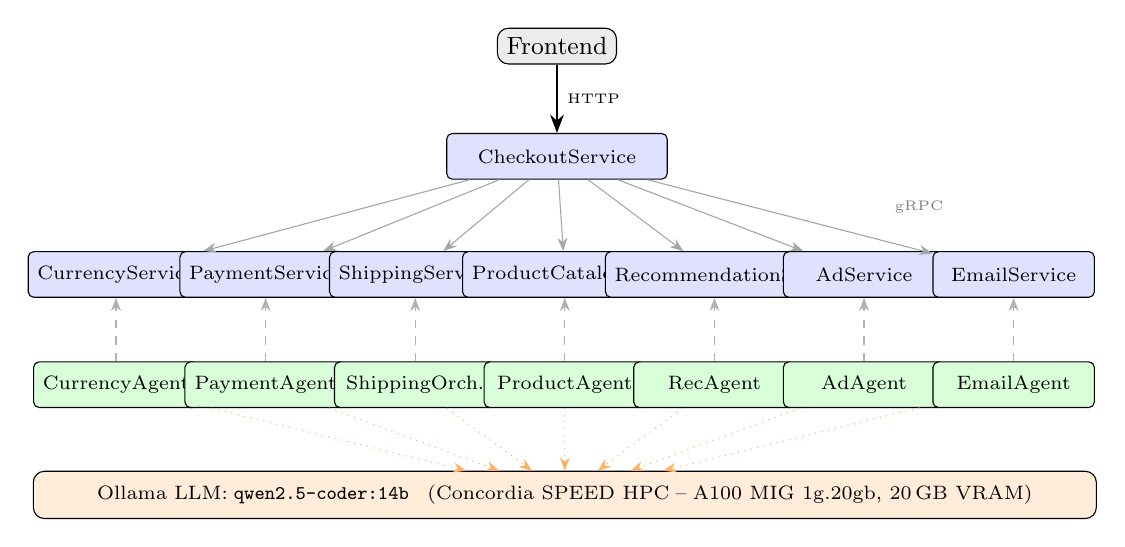
\begin{tikzpicture}[
  svc/.style={draw,fill=blue!12,rounded corners=2pt,
    minimum width=2.05cm,minimum height=0.58cm,
    font=\scriptsize,align=center},
  agt/.style={draw,fill=green!15,rounded corners=2pt,
    minimum width=2.05cm,minimum height=0.58cm,
    font=\scriptsize,align=center},
  >=Stealth
]
\node[draw,fill=gray!15,rounded corners,font=\small] (ui)
  at (0, 3.5) {Frontend};
\node[svc,minimum width=2.8cm] (cs)
  at (0, 2.1) {CheckoutService};
\node[svc] (curr)  at (-5.6, 0.6) {CurrencyService};
\node[svc] (pay)   at (-3.7, 0.6) {PaymentService};
\node[svc] (ship)  at (-1.8, 0.6) {ShippingService};
\node[svc] (prod)  at ( 0.1, 0.6) {ProductCatalogSvc};
\node[svc] (rec)   at ( 2.0, 0.6) {RecommendationSvc};
\node[svc] (ad)    at ( 3.9, 0.6) {AdService};
\node[svc] (email) at ( 5.8, 0.6) {EmailService};
\node[agt] (curra)  at (-5.6, -0.8) {CurrencyAgent};
\node[agt] (paya)   at (-3.7, -0.8) {PaymentAgent};
\node[agt] (shipa)  at (-1.8, -0.8) {ShippingOrch.};
\node[agt] (proda)  at ( 0.1, -0.8) {ProductAgent};
\node[agt] (reca)   at ( 2.0, -0.8) {RecAgent};
\node[agt] (ada)    at ( 3.9, -0.8) {AdAgent};
\node[agt] (emaila) at ( 5.8, -0.8) {EmailAgent};
\node[draw,fill=orange!15,rounded corners,font=\scriptsize,
      minimum width=13.5cm,minimum height=0.6cm] (llm)
  at (0.1, -2.2)
  {Ollama LLM:\;\texttt{qwen2.5-coder:14b}
   \enspace(Concordia SPEED HPC\;--\;A100 MIG 1g.20gb, 20\,GB VRAM)};
\draw[->,thick] (ui) -- (cs) node[midway,right,font=\tiny] {HTTP};
\foreach \x in {curr,pay,ship,prod,rec,ad,email}
  \draw[->,gray!70,thin] (cs) -- (\x);
\node[font=\tiny,gray] at (4.6,1.45) {gRPC};
\foreach \x/\y in {curr/curra,pay/paya,ship/shipa,prod/proda,
                   rec/reca,ad/ada,email/emaila}{
  \draw[->,dashed,gray!60,thin] (\y) -- (\x);
  \draw[->,dotted,orange!60,thin] (\y) -- (llm);
}
\end{tikzpicture}
\caption{LLM-MAS system architecture. Microservices (blue) serve
\texttt{CheckoutService} via gRPC (solid arrows). Agent wrappers (green)
orchestrate each microservice via LangGraph\,/\,ReAct (dashed) and share a
single Ollama LLM backend (orange, dotted).}
\label{fig:architecture}
\end{figure*}

\subsection{Fault Taxonomy}
We use MAST-aligned categories and business-logic scenarios:
\begin{itemize}
  \item \textbf{FM-1.2}: Incorrect task decomposition
  \item \textbf{FM-2.2}: Hallucinated tool output / fabricated carrier data
  \item \textbf{FM-2.5}: Ignored downstream agent input (stale cost)
  \item \textbf{FM-3.1}: Premature termination
  \item \textbf{BL}: SHIPMENT\_LOST, INVENTORY\_MISMATCH, VENDOR\_NEGOTIATION,
        CUSTOMER\_ESCALATION, REFUND\_REASONING, COMPLIANCE\_AMBIGUITY
\end{itemize}

% ═════════════════════════════════════════════════════════════════════════════
\section{Failure Injection and Analysis Workflow}
% ═════════════════════════════════════════════════════════════════════════════

Per advisor and team guidance, the study follows four phases:
(1)~define the injection and analysis workflow,
(2)~execute all listed scenarios with observation and root cause analysis,
(3)~complete Google-bench first, then Retail-bench, and
(4)~merge team results to answer all research questions.
Fig.~\ref{fig:workflow} illustrates the full pipeline.

\begin{figure*}[!t]
\centering
\resizebox{0.95\textwidth}{!}{%
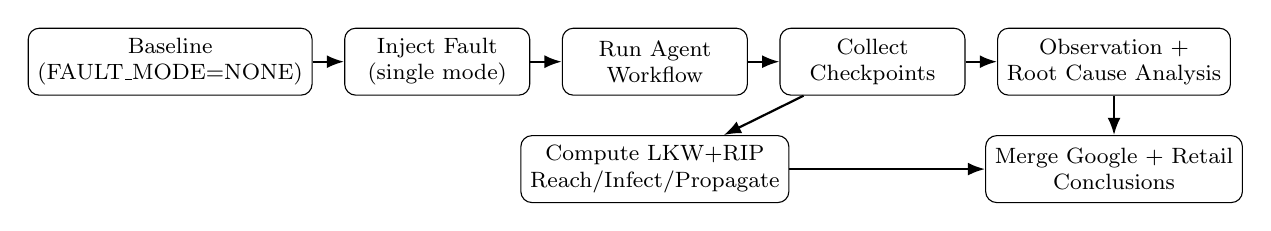
\begin{tikzpicture}[
  node distance=5mm and 4mm,
  box/.style={draw, rounded corners, align=center,
              minimum width=2.35cm, minimum height=0.85cm, font=\footnotesize},
  arr/.style={-{Latex[length=2.2mm]}, thick}
]
\node[box] (baseline) {Baseline\\(FAULT\_MODE=NONE)};
\node[box, right=of baseline] (inject) {Inject Fault\\(single mode)};
\node[box, right=of inject]   (run)    {Run Agent\\Workflow};
\node[box, right=of run]      (trace)  {Collect\\Checkpoints};
\node[box, below=of run]      (rip)    {Compute LKW+RIP\\Reach/Infect/Propagate};
\node[box, right=of trace]    (rca)    {Observation +\\Root Cause Analysis};
\node[box, below=of rca]      (merge)  {Merge Google + Retail\\Conclusions};

\draw[arr] (baseline) -- (inject);
\draw[arr] (inject)   -- (run);
\draw[arr] (run)      -- (trace);
\draw[arr] (trace)    -- (rca);
\draw[arr] (trace)    -- (rip);
\draw[arr] (rip)      -- (merge);
\draw[arr] (rca)      -- (merge);
\end{tikzpicture}%
}
\caption{Failure injection and analysis workflow used in this study.}
\label{fig:workflow}
\end{figure*}

% ═════════════════════════════════════════════════════════════════════════════
\section{Metrics and Definitions}
% ═════════════════════════════════════════════════════════════════════════════

For each run, we record the checkpoint sequence and compute:
\begin{itemize}
  \item \textbf{Reachability}: checkpoints reached under the fault mode.
  \item \textbf{Infection point}: first checkpoint with semantically deviant
        data.
  \item \textbf{Propagation depth}: number of downstream steps absent in the
        fault trace.
  \item \textbf{Steps lost}: checkpoints present in the baseline but missing
        in the faulty run.
\end{itemize}

Let $B$ be the baseline checkpoint set and $F$ the faulty checkpoint set:
\begin{equation}
  \mathrm{StepsLost} = B \setminus F
\end{equation}
\begin{equation}
  \mathrm{PropagationDepth} = \lvert B \setminus F \rvert
\end{equation}

% ═════════════════════════════════════════════════════════════════════════════
\section{Experimental Setup}
% ═════════════════════════════════════════════════════════════════════════════

\subsection{Compute Environment}
Runs are executed on Concordia SPEED HPC with dedicated compute allocation.
Runtime is controlled via timeout, retry, token, and iteration limits to reduce
variance. The ShippingService Retail-bench campaign uses an NVIDIA A100-SXM4-80GB
in MIG mode (1g.20gb slice, 20\,GB VRAM) with \texttt{qwen2.5-coder:14b} (9\,GB
model weight, full GPU inference via Ollama).

\subsection{Execution Protocol}
\begin{enumerate}
  \item Run NONE baseline for each scenario pair.
  \item Run one fault mode at a time.
  \item Repeat for Google-bench (ShippingService, \texttt{llama3.2:1b}),
        then Retail-bench (ShippingService, \texttt{qwen2.5-coder:14b}); six
        deterministic agents use \texttt{USE\_LLM=false} throughout.
  \item Mark timeout traces as INCONCLUSIVE; rerun where feasible.
\end{enumerate}

\subsection{Agent Execution Modes}

\begin{itemize}
  \item \textbf{Six deterministic agents} (Payment, Currency, Email,
        ProductCatalog, Recommendation, Ad): fault injection tests call the
        agent's business-logic method directly, bypassing the LangGraph router
        and LLM inference call entirely. \texttt{USE\_LLM=false} is hardcoded
        in all test runners. These agents validate the correctness of the
        LKW+RIP instrumentation framework on deterministic Python code.
  \item \textbf{ShippingService}: the sole live-LLM agent. The full LangGraph
        ReAct loop is exercised with \texttt{qwen2.5-coder:14b} on SPEED HPC.
        Fault injection occurs at the Final Answer intercept, tool-dispatch, and
        post-agent metadata layers to be observable regardless of single-pass
        model behaviour.
\end{itemize}

\subsection{Instrumentation and Structural Fixes}
During the study, two structural issues were identified and resolved. First,
the shipping agent and service files were co-located in a single directory
(\texttt{shippingservice/}), whereas every other service in the system maintains
a dedicated agent folder (e.g., \texttt{paymentagent/}, \texttt{cart-agent/}).
This co-location caused fault-injection hooks to share scope with the gRPC
service layer, blurring the agent/service propagation boundary. The agent logic
was reorganised into a dedicated \texttt{shippingagent/} module, restoring the
separation pattern used by all other services.

Second, HITL intervention points were initially identified by manual trace
inspection. To remove this bottleneck, we implemented \texttt{hitl\_detector.py},
an automated classifier that parses LKW checkpoint evidence files and assigns
each fault scenario to one of the three intervention tiers defined in
Section~\ref{sec:rq4}. The detector confirmed all scenario classifications
without manual inspection.

% ═════════════════════════════════════════════════════════════════════════════
\section{Results: Google and Retail Benchmarks}
% ═════════════════════════════════════════════════════════════════════════════

\subsection{Google Bench}

Table~\ref{tab:google_results} reports the four executed fault scenarios for the
Google-bench shipping workflow using \texttt{llama3.2:1b}. Elapsed time is the
end-to-end wall-clock duration of each agent run on Concordia SPEED HPC.

\begin{table*}[!t]
\centering
\caption{Validated Google-bench fault-injection observations (\texttt{llama3.2:1b}).}
\label{tab:google_results}
\scriptsize
\setlength{\tabcolsep}{3pt}
\renewcommand{\arraystretch}{1.15}
\resizebox{\textwidth}{!}{%
\begin{tabular}{p{1.6cm}p{1.6cm}p{2.1cm}p{1.6cm}p{2.8cm}p{3.6cm}p{3.8cm}}
\toprule
Scenario & Elapsed (ms) & Infection Point & Propagation Depth & Steps Lost
         & Observation Summary & Root Cause Analysis \\
\midrule
FM-3.1
  & 454858.4
  & QUOTE\_DONE
  & 1
  & CARRIER\_DONE, ESCALATION\_CHECK
  & Premature final answer injected with tracking\_id=PREMATURE-0000;
    carrier-selection path terminated early.
  & Initial iteration-gated trigger failed with single-pass model behaviour.
    Fixed by intercepting any Final Answer regardless of iteration count. \\
\midrule
FM-1.2
  & 374918.3
  & SAVE\_DONE
  & 2
  & CARRIER\_DONE, TRACKING\_DONE, ESCALATION\_CHECK
  & Corrupted planning plus incomplete-path handling produced
    tracking\_id=INCOMPLETE-0000 and removed downstream stages.
  & Prompt-only corruption was absorbed by model priors; deterministic
    behaviour required dispatch-level and final-answer normalisation logic. \\
\midrule
FM-2.2
  & 455954.8
  & QUOTE\_DONE (cost=0 artifact); carrier hallucination confirmed at CARRIER\_DONE
  & 0
  & None
  & Fallback injection applied: carrier replaced with SpeedyShip,
    service\_level=ultra-express. Flow completed all 7 checkpoints.
    Infection surfaced via cost anomaly at QUOTE\_DONE.
  & Model output was non-canonical JSON; final-answer-level patch skipped.
    Ship-order normalisation fallback enforced carrier substitution. Silent
    hallucination not detectable from step trace alone --- requires checkpoint
    data inspection. \\
\midrule
FM-2.5
  & 453759.3
  & CARRIER\_DONE
  & 0
  & None
  & Fallback injection applied: stale cost 4.99 replaced real quoted value (0.00).
    All checkpoints reached. Carrier selection was recorded with wrong financial
    input.
  & Single-pass model output bypassed tool-level injection. Normalisation
    fallback enforced stale cost overwrite and set ignored\_downstream\_quote=True
    flag. Flow completed silently --- highest latent business risk among executed
    faults. \\
\bottomrule
\end{tabular}%
}
\end{table*}

\subsection{Retail Bench: ShippingService}

Table~\ref{tab:retail_results} presents the full Retail-bench campaign using
\texttt{qwen2.5-coder:14b} on SPEED HPC (A100 MIG, 20\,GB VRAM). All scenarios
use the seven-step checkpoint set: \texttt{TASK\_START}, \texttt{QUOTE\_DONE},
\texttt{CARRIER\_DONE}, \texttt{TRACKING\_DONE}, \texttt{SAVE\_DONE},
\texttt{ESCALATION\_CHECK}, \texttt{FINAL\_ANSWER}.

\begin{table*}[!t]
\centering
\caption{LKW+RIP fault-injection results for the ShippingService Retail Bench
  (\texttt{qwen2.5-coder:14b}, Concordia SPEED HPC A100 MIG 1g.20gb).
  \emph{Infection Point} is the first LKW checkpoint at which a data deviation
  from the fault-free baseline is detected.
  \emph{Propagation Depth} counts the number of expected downstream steps absent
  in the fault trace (computed against the instrumented expected-steps set).
  $\dagger$~See footnote regarding known instrumentation defect for FM-3.1.
  $\ddagger$~INCONCLUSIVE due to LLM inference timeout (577\,s); see Limitation~L2.}
\label{tab:retail_results}
\scriptsize
\setlength{\tabcolsep}{3pt}
\renewcommand{\arraystretch}{1.15}
\resizebox{\textwidth}{!}{%
\begin{tabular}{p{1.6cm}p{1.8cm}p{2.6cm}p{2.0cm}p{1.5cm}p{3.7cm}p{3.7cm}}
\toprule
Scenario & Injected At & Infection Point & Propagation Depth & Steps Lost
         & Observation Summary & Root Cause Analysis \\
\midrule
FM-3.1 Premature Termination
  & ReAct Final Answer intercept
  & \texttt{QUOTE\_DONE}
  & 1$^\dagger$
  & \texttt{CARRIER\_DONE}$^\dagger$
  & Agent returned \texttt{PREMATURE-0000} before carrier selection;
    \texttt{CARRIER\_DONE} absent from trace; \texttt{QUOTE\_DONE} and
    \texttt{TRACKING\_DONE} reached via post-injection normalisation with
    placeholder values; \texttt{SAVE\_DONE} recorded with
    \texttt{premature\_termination} reason. Elapsed: 44\,799\,ms.
  & \texttt{qwen2.5-coder:14b} completes the full workflow in a single LLM
    call, bypassing tool-dispatch-level injection; Final Answer interception
    is the only reliable injection layer for single-pass models.
    \texttt{ESCALATION\_CHECK} also absent but excluded from expected-steps
    set (instrumentation defect; see Limitation~L3). \textbf{Classification: Partial TP.} \\
\midrule
FM-1.2 Incomplete Task Spec
  & Task-spec mutation + tool dispatch block
  & \texttt{SAVE\_DONE}
  & 2
  & \texttt{CARRIER\_DONE}, \texttt{TRACKING\_DONE}, \texttt{ESC\_CHECK}
  & Corrupted task spec omitted carrier and tracking instructions; blocked tool
    calls returned errors; Final Answer contained \texttt{INCOMPLETE-0000};
    three downstream checkpoints absent.
  & Task-spec corruption removes planning context for carrier and tracking steps;
    dispatch-level blocking reinforces the gap; the agent cannot reconstruct
    steps absent from the corrupted specification. \textbf{Classification: TP.} \\
\midrule
FM-2.2 Hallucinated Carrier
  & Final Answer intercept
  & \texttt{CARRIER\_DONE}
  & 0
  & None
  & Carrier field silently replaced with unregistered \emph{SpeedyShip}; all
    seven LKW steps reached; no agent-level detection, rejection, or workflow
    deviation.
  & Single-pass model output bypasses tool-dispatch injection; Final Answer
    patch guarantees the hallucinated carrier surfaces regardless of the model's
    independent selection; no downstream guard validates carrier legitimacy.
    \textbf{Classification: TP.} \\
\midrule
FM-2.5 Stale Quote Ignored
  & Final Answer intercept + \texttt{ship\_order} fallback
  & \texttt{CARRIER\_DONE}
  & 0
  & None
  & Cost silently overridden to stale \$4.99; \texttt{ignored\_downstream\_quote=True}
    flag set at \texttt{CARRIER\_DONE}; full step reachability preserved with no
    agent alert or error.
  & Live quote bypassed by a pre-injected stale cost; absence of a
    quote-consistency invariant in the carrier-selection path allows silent cost
    absorption with no observable agent reaction. \textbf{Classification: TP.} \\
\midrule
BL-Shipment Lost
  & \texttt{ship\_order} MongoDB save bypass
  & --- (step absent)
  & 1
  & \texttt{SAVE\_DONE}
  & \texttt{SAVE\_DONE} checkpoint wholly absent from fault trace; shipment
    processed and tracking ID issued, but record never persisted to MongoDB;
    silent data-loss with no error raised.
  & The save-skip fault removes \texttt{SAVE\_DONE} from the trace entirely
    rather than corrupting its contents; this fault class manifests as step
    absence rather than data deviation, so infection point is undefined and
    propagation captures the loss. \textbf{Classification: Partial TP.} \\
\midrule
BL-Inventory Mismatch
  & Pre-task item quantity inflation (\texttt{ship\_order})
  & \texttt{QUOTE\_DONE}
  & 0
  & None
  & Item quantities doubled before agent task construction;
    \texttt{item\_count\_inflated=True} flag detected at first quote checkpoint;
    downstream carrier selection and tracking completed normally on inflated data.
  & Corruption precedes the agent loop; all subsequent model computations
    silently use inflated quantities; no input-validation gate exists between
    item receipt and task construction. \textbf{Classification: TP.} \\
\midrule
BL-Vendor Negotiation
  & Final Answer intercept + \texttt{ship\_order} fallback
  & \texttt{CARRIER\_DONE}
  & 0
  & None
  & Carrier forced to \emph{PremiumExpress} overnight service;
    \texttt{forced\_vendor=True} flag recorded at \texttt{CARRIER\_DONE};
    agent completed the full order without detecting the expensive substitution.
  & Preferred-carrier unavailability injected at the output layer; agent lacks a
    post-selection check to validate the chosen carrier against negotiated rates
    or cost thresholds, enabling silent vendor substitution.
    \textbf{Classification: TP.} \\
\midrule
BL-Customer Escalation
  & Post-agent metadata injection (\texttt{ship\_order})
  & \texttt{ESCALATION\_CHECK}
  & 0
  & None
  & \texttt{escalation\_required=True} injected into \texttt{ESCALATION\_CHECK}
    metadata after agent loop completion; high-risk order silently persisted
    without human review, alert, or workflow halt.
  & Escalation flag injected after model completion; the agent has no
    \texttt{ESCALATION\_CHECK} guard in its execution path to interrupt or divert
    high-risk shipments before persistence. \textbf{Classification: TP.} \\
\midrule
BL-Refund Reasoning
  & Post-agent cost negation (\texttt{ship\_order})
  & \texttt{QUOTE\_DONE}
  & 0
  & None
  & \texttt{cost\_usd} forced to $-$0.0 (IEEE~754 negative zero); sign-bit
    detection via \texttt{math.copysign} confirmed corruption at
    \texttt{QUOTE\_DONE}; agent proceeded to carrier selection and tracking
    without rejecting the invalid cost.
  & Refund-required condition simulated by negating cost; agent lacks a
    non-negative cost invariant; negative-zero is numerically equal to zero,
    requiring sign-bit inspection to distinguish intentional corruption from a
    zero-cost artefact. \textbf{Classification: TP.} \\
\midrule
BL-Compliance Ambiguity$^\ddagger$
  & Pre-task address tagging (\texttt{compliance\_jurisdiction=UNKNOWN})
  & \texttt{SAVE\_DONE} (partial; timeout)
  & 3
  & \texttt{QUOTE\_DONE}, \texttt{CARRIER\_DONE}, \texttt{TRACKING\_DONE}
  & Under \texttt{qwen2.5-coder:14b}, the LLM inference call for the
    compliance-ambiguous task exceeded the 120\,s HTTP read timeout (total
    elapsed: 577\,682\,ms); \texttt{FINAL\_ANSWER} recorded a connection
    timeout error; three checkpoints absent; \texttt{SAVE\_DONE} reached with
    \texttt{reason=benchmark\_mode}. Distinct from \texttt{llama3.2:1b}
    behaviour (loop exhaustion in 4 iterations) --- timeout occurs during
    the first LLM call, indicating the compliance reasoning task exceeds
    available inference time regardless of model scale.
  & Compliance jurisdiction ambiguity generates a semantically complex
    reasoning task that exhausts available LLM inference time at both tested
    model scales; the 14B model requires $>$120\,s per inference call under
    this scenario; explicit compliance-gating logic is needed outside the
    LLM reasoning loop to avoid blocking the workflow.
    \textbf{Classification: INCONCLUSIVE (LLM inference timeout).} \\
\midrule
NONE Baseline
  & ---
  & None
  & 0
  & None
  & All expected checkpoints reached; no infection signal; agent completes
    order normally.
  & Clean baseline. \textbf{Classification: TN.} \\
\bottomrule
\multicolumn{7}{p{17cm}}{$^\dagger$\,Depth reported as 1 (\texttt{CARRIER\_DONE} only); \texttt{ESCALATION\_CHECK} also absent but excluded from expected-steps set --- known instrumentation defect (Limitation~L3). Actual absent steps: 2.} \\
\multicolumn{7}{p{17cm}}{$^\ddagger$\,INCONCLUSIVE due to LLM inference timeout at both \texttt{llama3.2:1b} (loop exhaustion) and \texttt{qwen2.5-coder:14b} (HTTP read timeout $>$120\,s). See Limitation~L2.}
\end{tabular}%
}
\end{table*}

% ═════════════════════════════════════════════════════════════════════════════
\section{Results: Agent-Level Fault Injection}
% ═════════════════════════════════════════════════════════════════════════════

We extend the fault-injection campaign to six standalone Python-based agent
services in the LLM-MAS architecture. Each agent is instrumented with LKW
checkpoints; gRPC dependencies are replaced with controlled mocks so that all
faults execute deterministically without network I/O. \emph{The LLM inference
path is bypassed in all six agents} (\texttt{USE\_LLM=false}); these results
validate the correctness of the LKW+RIP instrumentation framework on
deterministic code, not LLM-based fault detection capability (see
Limitation~L1).

% ── PaymentAgent ─────────────────────────────────────────────────────────────
\subsection{PaymentAgent}

Checkpoints: \texttt{TASK\_START} $\to$ \texttt{CARD\_VALIDATED} $\to$
\texttt{CHARGE\_DONE} $\to$ \texttt{SAVE\_DONE} $\to$ \texttt{FINAL\_ANSWER}.
Table~\ref{tab:payment_results} reports all nine fault modes.

\begin{table*}[!t]
\centering
\caption{PaymentAgent LKW+RIP Fault-Injection Results.
  \emph{Infection Point} is the first LKW checkpoint at which a data deviation
  from the fault-free baseline is detected.
  \emph{Propagation Depth} counts downstream steps absent in the fault trace.
  \emph{Steps Lost} lists checkpoints present in the NONE baseline but absent
  in the fault run.}
\label{tab:payment_results}
\scriptsize
\setlength{\tabcolsep}{3pt}
\renewcommand{\arraystretch}{1.15}
\begin{tabularx}{\textwidth}{J{1.4cm}J{1.9cm}J{1.7cm}cJ{1.4cm}KK}
\toprule
Scenario & Injected At & Infection Point & Propagation Depth & Steps Lost
         & Observation Summary & Root Cause Analysis \\
\midrule
NONE Baseline
  & ---
  & ---
  & 0
  & ---
  & All 5/5 checkpoints reached; card validates correctly; charge and save
    execute without error.
  & Clean baseline; \texttt{charge\_payment()} called with correct parameters;
    \texttt{save\_transaction()} persists result. \\
\midrule
FM-3.1 Premature Termination
  & \texttt{run()} early return
  & \texttt{FINAL\_ANSWER}
  & 3
  & \texttt{CARD\_VALIDATED}, \texttt{CHARGE\_DONE}, \texttt{SAVE\_DONE}
  & Agent returned \texttt{PREMATURE-0000} before charge execution; three
    downstream checkpoints absent; transaction neither processed nor persisted.
  & \texttt{maybe\_premature\_termination()} intercepts control before
    \texttt{charge\_payment()} is called; no charge, no save, no transaction
    record produced. \\
\midrule
FM-2.2 Hallucinated Transaction ID
  & \texttt{charge\_payment} return intercept
  & \texttt{CHARGE\_DONE}
  & 0
  & None
  & Real UUID replaced with \texttt{FAKE-TXN-*}; all five checkpoints reached;
    hallucinated ID saved to MongoDB with no rejection.
  & No downstream guard validates transaction ID format or origin; fabricated
    ID is accepted and persisted identically to a real charge result. \\
\midrule
FM-2.5 Amount Ignored
  & Pre-charge amount replacement
  & \texttt{CARD\_VALIDATED}
  & 0
  & None
  & Charge amount silently inflated from \$10.99 to \$30.99 before
    \texttt{charge\_payment()}; all steps completed; overcharge persisted with
    no alert.
  & Amount passed to \texttt{charge\_payment()} is not validated against the
    original request; no pre-charge invariant check exists in the execution
    path. \\
\midrule
FM-1.2 Validation Bypassed
  & \texttt{charge\_payment} validation gate
  & \texttt{CARD\_VALIDATED}
  & 0
  & None
  & All card validation checks skipped via \texttt{\_bypass\_validation} flag;
    invalid or expired cards accepted and charged; full step reachability
    preserved.
  & Validation logic is conditional on a request-level flag; no secondary
    verification layer exists to catch bypassed validation before charge
    execution. \\
\midrule
BL-Transaction Lost
  & \texttt{save\_transaction} bypass
  & \texttt{SAVE\_DONE}
  & 0
  & None
  & Charge succeeded and transaction ID issued, but \texttt{save\_transaction()}
    silently skipped; \texttt{save\_skipped=True} recorded at \texttt{SAVE\_DONE};
    no error raised.
  & Persistence is gated by a single boolean check with no fallback; a failed or
    bypassed save produces no exception, leaving the transaction unrecorded. \\
\midrule
BL-Double Charge
  & \texttt{save\_transaction} payload injection
  & \texttt{SAVE\_DONE}
  & 0
  & None
  & \texttt{double\_charge=True} and \texttt{duplicate\_of} markers injected
    into save payload; duplicate transaction persisted without deduplication
    check or alert.
  & No idempotency key or duplicate-transaction guard exists in the save path;
    the agent accepts and persists a flagged duplicate without triggering any
    intervention. \\
\midrule
BL-Amount Tampering
  & Pre-charge amount inflation
  & \texttt{CARD\_VALIDATED}
  & 0
  & None
  & Charge amount inflated $3\times$ before processing;
    \texttt{amount\_tampered=True} recorded at \texttt{CARD\_VALIDATED};
    inflated amount persisted to MongoDB silently.
  & Equivalent to FM-2.5 at the injection layer; absence of a request-to-charge
    amount consistency invariant allows silent over-billing with no observable
    workflow deviation. \\
\midrule
BL-Card Declined
  & \texttt{CreditCardError} injection
  & \texttt{FINAL\_ANSWER}
  & 3
  & \texttt{CARD\_VALIDATED}, \texttt{CHARGE\_DONE}, \texttt{SAVE\_DONE}
  & Valid VISA card forced to decline; \texttt{CreditCardError} raised before
    charge; three downstream checkpoints absent;
    \texttt{forced\_decline=True} recorded at \texttt{FINAL\_ANSWER}.
  & Decline injected via \texttt{maybe\_force\_decline()} before
    \texttt{charge\_payment()}; no retry logic or human-escalation path exists
    for forced PSP rejections. \\
\bottomrule
\end{tabularx}
\end{table*}

% ── CurrencyAgent ─────────────────────────────────────────────────────────────
\subsection{CurrencyAgent}

Checkpoints: \texttt{TASK\_START} $\to$ \texttt{CONVERT\_DONE} $\to$
\texttt{FINAL\_ANSWER}. Table~\ref{tab:currency-fault} reports all nine fault
modes.

\begin{table*}[!t]
\centering
\caption{CurrencyAgent LKW+RIP Fault-Injection Results.}
\label{tab:currency-fault}
\scriptsize
\setlength{\tabcolsep}{3pt}
\renewcommand{\arraystretch}{1.15}
\begin{tabularx}{\textwidth}{J{1.4cm}J{1.9cm}J{1.7cm}cJ{1.4cm}KK}
\toprule
\textbf{Scenario} & \textbf{Injected At} & \textbf{Infection Point}
  & \textbf{Prop.\ Depth} & \textbf{Steps Lost}
  & \textbf{Observation Summary} & \textbf{Root Cause Analysis} \\
\midrule
NONE Baseline
  & ---  & ---  & 0  & ---
  & 9.23\,EUR returned correctly; all three checkpoints reached; gRPC mock
    returns \texttt{units=9, nanos=230000000}.
  & Clean baseline; \texttt{CurrencyGrpcClient.convert()} called with correct
    parameters; no anomalies detected. \\
FM-3.1 Premature Termination
  & \texttt{run()} early return before \texttt{client.convert()}
  & \texttt{FINAL\_ANSWER}  & 1  & \texttt{CONVERT\_DONE}
  & \texttt{maybe\_premature\_termination()} intercepts control;
    \texttt{currency\_code=PREMATURE}, \texttt{units=0} returned;
    \texttt{CONVERT\_DONE} absent from LKW trace.
  & No guard on gRPC call completion; \texttt{run()} returns immediately on
    fault flag without invoking the conversion stub; single downstream
    checkpoint lost. \\
FM-2.2 Hallucinated Result
  & \texttt{convert()} return intercept
  & \texttt{CONVERT\_DONE}  & 0  & ---
  & \texttt{maybe\_hallucinate\_result()} replaces gRPC response with
    \texttt{units=1337, nanos=420000000}; real result suppressed;
    \texttt{hallucinated=True} at \texttt{CONVERT\_DONE}; all steps reached.
  & Single-pass conversion path; no downstream validation of returned Money
    fields; fabricated amounts accepted and propagated to \texttt{FINAL\_ANSWER}
    without range or format checks. \\
FM-2.5 Amount Ignored
  & Pre-convert amount replacement
  & \texttt{CONVERT\_DONE}  & 0  & ---
  & \texttt{maybe\_tamper\_amount()} multiplies \texttt{units} $5\times$
    ($10 \to 50$) before \texttt{client.convert()};
    \texttt{amount\_tampered=True} in checkpoint; gRPC dispatched with inflated
    input.
  & No pre-call consistency invariant between request units and execution units;
    absence of input-validation gate before gRPC dispatch allows silent
    overcharge propagation. \\
FM-1.2 Wrong Currency Routing
  & \texttt{to\_currency} param swap
  & \texttt{CONVERT\_DONE}  & 0  & ---
  & \texttt{maybe\_swap\_currency()} changes \texttt{EUR}$\to$\texttt{JPY}
    before gRPC call; \texttt{currency\_swapped=True}; gRPC invoked with wrong
    target; result returned to caller silently.
  & Target currency is a plain string parameter with no contract enforcement;
    no caller-side verification of currency pair legality before dispatch. \\
BL-RATE-MANIP Rate Inflated
  & Post-gRPC result inflate
  & \texttt{CONVERT\_DONE}  & 0  & ---
  & \texttt{maybe\_manipulate\_rate()} inflates returned \texttt{units} $10\times$
    ($9 \to 90$); \texttt{rate\_manipulated=True};
    \texttt{original\_units=9} preserved in checkpoint.
  & Conversion result passes through agent layer without cross-validation against
    known exchange-rate bounds; agent acts as an unaudited intermediary between
    gRPC data and caller. \\
BL-CURR-UNAVAIL Unsupported
  & Pre-gRPC error injection
  & \texttt{FINAL\_ANSWER}  & 1  & \texttt{CONVERT\_DONE}
  & \texttt{maybe\_simulate\_unavailable()} raises \texttt{RuntimeError} before
    gRPC call; \texttt{unavailable=True}; \texttt{CONVERT\_DONE} absent; error
    propagated to \texttt{FINAL\_ANSWER}; structurally equivalent to FM-3.1.
  & Service treats unsupported-currency as terminal; no retry, fallback
    currency, or graceful degradation path; one structural step lost with no
    recovery option. \\
BL-STALE-RATE Cached Rate
  & Post-gRPC cache replace
  & \texttt{CONVERT\_DONE}  & 0  & ---
  & \texttt{maybe\_inject\_stale\_rate()} replaces live response with cached
    \texttt{units=0, nanos=850000000} dated \texttt{2026-01-01};
    \texttt{stale\_rate=True}; gRPC called but result discarded.
  & No cache-invalidation guard or timestamp comparison between gRPC response
    and returned value; stale rate accepted silently with no observable
    workflow deviation. \\
BL-CONV-OVERFLOW Overflow Value
  & Post-convert value inject
  & \texttt{CONVERT\_DONE}  & 0  & ---
  & \texttt{maybe\_overflow\_result()} sets \texttt{units=}$2^{53}$
    (\texttt{9007199254740992}), \texttt{nanos=999999999};
    \texttt{overflow=True} at \texttt{CONVERT\_DONE}; extreme value propagated
    without rejection.
  & No numeric bounds validation on \texttt{Money.units} field; IEEE\,754
    double-precision overflow accepted as a valid conversion result; absent
    overflow guard at Money serialisation layer. \\
\bottomrule
\end{tabularx}
\end{table*}

% ── EmailServiceAgent ─────────────────────────────────────────────────────────
\subsection{EmailServiceAgent}

Checkpoints: \texttt{TASK\_START} $\to$ \texttt{EMAIL\_GENERATED} $\to$
\texttt{EMAIL\_SENT} $\to$ \texttt{FINAL\_ANSWER}. Faults are injected across
both the LangGraph \texttt{run\_agent\_node} and
\texttt{send\_via\_microservice\_node}. Table~\ref{tab:email-fault} reports all
nine fault modes.

\begin{table*}[!t]
\centering
\caption{EmailServiceAgent LKW+RIP Fault-Injection Results.}
\label{tab:email-fault}
\scriptsize
\setlength{\tabcolsep}{3pt}
\renewcommand{\arraystretch}{1.15}
\begin{tabularx}{\textwidth}{J{1.4cm}J{1.9cm}J{1.7cm}cJ{1.4cm}KK}
\toprule
\textbf{Scenario} & \textbf{Injected At} & \textbf{Infection Point}
  & \textbf{Prop.\ Depth} & \textbf{Steps Lost}
  & \textbf{Observation Summary} & \textbf{Root Cause Analysis} \\
\midrule
NONE Baseline
  & ---  & ---  & 0  & ---
  & \texttt{email\_type=order\_confirmation}; subject correct;
    \texttt{body\_len=68}; \texttt{microservice\_status=sent}; all 4/4
    checkpoints reached.
  & Clean baseline; \texttt{generate\_email\_content()} returns structured
    content; \texttt{EmailServiceClient} sends via gRPC without error. \\
FM-3.1 Premature Termination
  & \texttt{run\_agent\_node()} early return
  & \texttt{FINAL\_ANSWER}  & 2
  & \texttt{EMAIL\_GENERATED}, \texttt{EMAIL\_SENT}
  & \texttt{maybe\_premature\_termination()} triggers before
    \texttt{generate\_email\_content()}; \texttt{email\_type=PREMATURE\_TERMINATION};
    body empty; \texttt{microservice\_status=skipped\_premature}; two
    checkpoints lost.
  & Highest propagation depth (2) in this agent's campaign; both generation and
    delivery nodes skipped via state flag; no email produced or sent; premature
    flag propagates silently through LangGraph state. \\
FM-2.2 Hallucinated Email
  & \texttt{generate\_email\_content()} return intercept
  & \texttt{EMAIL\_GENERATED}  & 0  & ---
  & \texttt{maybe\_hallucinate\_email()} replaces real content with subject
    \emph{``CONGRATULATIONS! You've won a prize''} and phishing-style body;
    \texttt{hallucinated=True}; email delivered to real recipient via gRPC.
  & LangGraph node does not validate subject or body content before forwarding
    to the send node; no content-policy or format guard between generation and
    delivery; malicious content reaches the email service. \\
FM-2.5 Recipient Ignored
  & Pre-generation address swap
  & \texttt{EMAIL\_GENERATED}  & 0  & ---
  & \texttt{maybe\_swap\_recipient()} replaces email with
    \texttt{wrong.address@devnull.test} before
    \texttt{generate\_email\_content()}; \texttt{recipient\_swapped=True};
    email dispatched to wrong address via gRPC.
  & Request dict passed by reference through graph state; no recipient binding
    from original order context to send step; the single email field in state
    is the sole delivery target with no cross-validation. \\
FM-1.2 Wrong Email Type
  & Email-type reclassification
  & \texttt{EMAIL\_GENERATED}  & 0  & ---
  & \texttt{maybe\_wrong\_email\_type()} changes
    \texttt{order\_confirmation}$\to$\texttt{promotional};
    \texttt{email\_type=promotional} persisted in state; subject unchanged;
    \texttt{type\_wrong=True}; send proceeds normally.
  & Classification occurs in a single function call with no downstream
    reconciliation; type label affects template selection without any contract
    between classification output and order context. \\
BL-SEND-SKIPPED Send Bypassed
  & \texttt{send\_via\_microservice\_node()} skip
  & \texttt{EMAIL\_SENT}  & 0  & ---
  & \texttt{maybe\_skip\_send()} bypasses gRPC call; content generated
    correctly; \texttt{microservice\_status=skipped\_fault};
    \texttt{EMAIL\_SENT} reached with \texttt{send\_skipped=True}; no delivery
    occurs.
  & Send step is a single boolean-gated gRPC call with no acknowledgment or
    retry; skipping produces a valid-looking completed state with no observable
    failure signal returned to the upstream caller. \\
BL-DOUBLE-SEND Duplicate Flag
  & \texttt{send\_via\_microservice\_node()} flag inject
  & \texttt{EMAIL\_SENT}  & 0  & ---
  & \texttt{maybe\_double\_send\_marker()} sets \texttt{double\_send=True} in
    \texttt{EMAIL\_SENT} checkpoint; gRPC executes normally; marker injected
    into LKW metadata only.
  & No idempotency key or deduplication guard in the send path;
    \texttt{double\_send} is a metadata-level fault; actual duplicate delivery
    requires a second gRPC call, represented here by the checkpoint flag. \\
BL-CORRUPT-BODY Body Corrupted
  & Post-generation body truncate
  & \texttt{EMAIL\_GENERATED}  & 0  & ---
  & \texttt{maybe\_corrupt\_body()} truncates body from 68 to 20 chars;
    \texttt{body\_len=20} at \texttt{EMAIL\_GENERATED};
    \texttt{corrupted=True}; truncated email delivered via gRPC without error.
  & No minimum-length or completeness validation on email body before dispatch;
    generate$\to$send pipeline has no structural integrity check on body
    content; truncated email sent silently. \\
BL-WRONG-CUSTOMER Wrong Name
  & Post-generation name replace
  & \texttt{EMAIL\_GENERATED}  & 0  & ---
  & \texttt{maybe\_wrong\_customer()} replaces \emph{Customer} with
    \emph{WRONG\_CUSTOMER} in body; \texttt{body\_len} increases to 80 chars;
    \texttt{wrong\_customer=True}; wrong name delivered via gRPC.
  & Customer name injected into body template at generation time with no
    post-generation identity verification; no binding between
    \texttt{order.customer\_name} and body content prior to send. \\
\bottomrule
\end{tabularx}
\end{table*}

% ── ProductCatalogAgent ───────────────────────────────────────────────────────
\subsection{ProductCatalogAgent}

Checkpoints: \texttt{TASK\_START} $\to$ \texttt{CATALOG\_DONE} $\to$
\texttt{FINAL\_ANSWER}. Three gRPC actions are covered:
\texttt{list\_products}, \texttt{get\_product}, \texttt{search\_products}.
Table~\ref{tab:catalog-fault} reports all nine fault modes.

\begin{table*}[!t]
\centering
\caption{ProductCatalogAgent LKW+RIP Fault-Injection Results.}
\label{tab:catalog-fault}
\scriptsize
\setlength{\tabcolsep}{3pt}
\renewcommand{\arraystretch}{1.15}
\begin{tabularx}{\textwidth}{J{1.4cm}J{1.9cm}J{1.7cm}cJ{1.4cm}KK}
\toprule
\textbf{Scenario} & \textbf{Injected At} & \textbf{Infection Point}
  & \textbf{Prop.\ Depth} & \textbf{Steps Lost}
  & \textbf{Observation Summary} & \textbf{Root Cause Analysis} \\
\midrule
NONE Baseline
  & ---  & ---  & 0  & ---
  & \texttt{list\_products} returns 2 products (PROD-001 Sunglasses, PROD-002
    Candle Holder); all 3/3 checkpoints reached; \texttt{price\_usd},
    \texttt{categories} fields correct.
  & Clean baseline; \texttt{ProductCatalog\allowbreak GrpcClient.\allowbreak list\_products()} invoked
    correctly; product dicts include all required fields. \\
FM-3.1 Premature Termination
  & \texttt{run()} early return before gRPC
  & \texttt{FINAL\_ANSWER}  & 1  & \texttt{CATALOG\_DONE}
  & \texttt{maybe\_premature\_termination()} intercepts before any gRPC call;
    returns \texttt{[]}; \texttt{CATALOG\_DONE} absent;
    \texttt{premature\_termination=True} at \texttt{FINAL\_ANSWER}.
  & No guard on gRPC call completion; action routing logic never reached; empty
    product list silently propagated to caller; one structural checkpoint lost. \\
FM-2.2 Hallucinated Products
  & Post-gRPC result replace
  & \texttt{CATALOG\_DONE}  & 0  & ---
  & \texttt{maybe\_hallucinate\_products()} replaces real list with
    \texttt{[\{"id":"HALLUCINATED-001","name":"Fabricated Product",
    "price\_usd":\{"units":9999\}\}]};
    \texttt{hallucinated=True} at \texttt{CATALOG\_DONE}.
  & No downstream validation of product ID format or existence against known
    catalog; fabricated product at \$9999 accepted and returned without catalog
    cross-reference or ID integrity check. \\
FM-2.5 Query Ignored
  & Pre-gRPC query replace
  & \texttt{CATALOG\_DONE}  & 0  & ---
  & \texttt{maybe\_tamper\_query()} replaces \emph{``list all products''} with
    \emph{``nonexistent\_item\_xyz''}; \texttt{query\_tampered=True};
    \texttt{search\_products("nonexistent\_item\_xyz")} dispatched to gRPC.
  & Query string is the sole routing input with no binding to the original
    request object; silent query substitution before gRPC dispatch goes
    undetected; mock returns original list regardless. \\
FM-1.2 Wrong Action Routing
  & Action routing swap
  & \texttt{CATALOG\_DONE}  & 0  & ---
  & \texttt{maybe\_swap\_action()} changes
    \texttt{list\_products}$\to$\texttt{search\_products};
    \texttt{action\_swapped=True}; different gRPC method invoked; search
    returns 1 product instead of 2; caller receives partial result.
  & Action routing is a single string comparison with no idempotency check;
    swapping list$\to$search changes the gRPC method but produces no observable
    error; silent partial result accepted. \\
BL-PRODUCT-MISSING Empty Catalog
  & Post-gRPC result clear
  & \texttt{CATALOG\_DONE}  & 0  & ---
  & \texttt{maybe\_remove\_products()} clears result to \texttt{[]};
    \texttt{count=0} at \texttt{CATALOG\_DONE}; gRPC was called successfully;
    result silently discarded; \texttt{FINAL\_ANSWER} receives empty catalog.
  & No minimum result-count validation between gRPC response and return path;
    empty list is structurally valid; silent data loss with no error raised or
    fallback triggered. \\
BL-PRICE-MANIP Prices Inflated
  & Post-gRPC price inflate $\times10$
  & \texttt{CATALOG\_DONE}  & 0  & ---
  & \texttt{maybe\_manipulate\_prices()} multiplies all
    \texttt{price\_usd.units} by 10; PROD-001: \texttt{units} $19\to190$;
    \texttt{price\_manipulated=True}; all other fields unchanged.
  & Price fields are mutable dicts passed by reference through agent layer; no
    immutability guarantee or price-bound validation between gRPC response and
    caller; silent $10\times$ inflation accepted. \\
BL-DUP-PRODUCT Duplicated
  & Post-gRPC list prepend
  & \texttt{CATALOG\_DONE}  & 0  & ---
  & \texttt{maybe\_duplicate\_product()} prepends first product; result count:
    $2\to3$; PROD-001 appears twice; \texttt{duplicated=True} at
    \texttt{CATALOG\_DONE}.
  & No deduplication or product-ID uniqueness check on returned catalog list;
    result accepted as-is from agent layer; duplicate entry propagated to caller
    silently. \\
BL-WRONG-CATEGORY Categories
  & Post-gRPC category override
  & \texttt{CATALOG\_DONE}  & 0  & ---
  & \texttt{maybe\_wrong\_category()} replaces all categories with
    \texttt{["WRONG\_CATEGORY"]}; PROD-001 had \texttt{["accessories"]},
    PROD-002 had \texttt{["home"]}; \texttt{category\_wrong=True}.
  & Category list is a mutable dict field with no schema enforcement after gRPC
    deserialisation; agent modifies categories in-place without triggering any
    validation or mismatch alert. \\
\bottomrule
\end{tabularx}
\end{table*}

% ── RecommendationAgent ───────────────────────────────────────────────────────
\subsection{RecommendationAgent}

Checkpoints: \texttt{TASK\_START} $\to$ \texttt{RECOMMEND\_DONE} $\to$
\texttt{FINAL\_ANSWER}. Both \texttt{get\_recommendations} and
\texttt{explain\_recommendations} share the same \texttt{\_fetch()} path and
\texttt{list\_recommendations} gRPC call.
Table~\ref{tab:recommendation-fault} reports all nine fault modes.

\begin{table*}[!t]
\centering
\caption{RecommendationAgent LKW+RIP Fault-Injection Results.}
\label{tab:recommendation-fault}
\scriptsize
\setlength{\tabcolsep}{3pt}
\renewcommand{\arraystretch}{1.15}
\begin{tabularx}{\textwidth}{J{1.4cm}J{1.9cm}J{1.7cm}cJ{1.4cm}KK}
\toprule
\textbf{Scenario} & \textbf{Injected At} & \textbf{Infection Point}
  & \textbf{Prop.\ Depth} & \textbf{Steps Lost}
  & \textbf{Observation Summary} & \textbf{Root Cause Analysis} \\
\midrule
NONE Baseline
  & ---  & ---  & 0  & ---
  & \texttt{list\_recommendations} returns
    \texttt{['PROD-042','PROD-017','PROD-009']}; \texttt{user\_id=user-abc123};
    all 3/3 checkpoints reached; output IDs disjoint from inputs.
  & Clean baseline; \texttt{Recommendation\allowbreak GrpcClient.\allowbreak list\_recommendations()}
    invoked with correct \texttt{user\_id} and \texttt{product\_ids}. \\
FM-3.1 Premature Termination
  & \texttt{\_fetch()} early return
  & \texttt{FINAL\_ANSWER}  & 1  & \texttt{RECOMMEND\_DONE}
  & \texttt{maybe\_premature\_termination()} returns \texttt{[]} before
    \texttt{list\_recommendations()}; \texttt{RECOMMEND\_DONE} absent;
    \texttt{recommended\_product\_ids=[]} in final state.
  & No guard on gRPC call completion; user and product context recorded at
    \texttt{TASK\_START} but never processed; empty recommendation list silently
    returned to caller with no error. \\
FM-2.2 Hallucinated IDs
  & Post-gRPC ID replace
  & \texttt{RECOMMEND\_DONE}  & 0  & ---
  & \texttt{maybe\_hallucinate\_recs()} replaces real IDs with
    \texttt{['HALLUCINATED-001',\allowbreak 'HALLUCINATED-002',\allowbreak 'HALLUCINATED-003']};
    \texttt{hallucinated=True}; gRPC called; real result discarded.
  & No downstream validation of returned product IDs against known catalog;
    fabricated IDs accepted; downstream product resolution will silently fail
    if these IDs are forwarded to \texttt{ProductCatalogService}. \\
FM-2.5 User ID Ignored
  & Pre-gRPC \texttt{user\_id} swap
  & \texttt{RECOMMEND\_DONE}  & 0  & ---
  & \texttt{maybe\_swap\_user\_id()} replaces
    \texttt{user-abc123}$\to$\texttt{WRONG\_USER\_000};
    \texttt{user\_id\_swapped=True}; gRPC called with wrong identity; mock
    returns same IDs regardless of identity.
  & \texttt{user\_id} is a plain string with no session-binding or identity
    verification before gRPC dispatch; wrong user's recommendation profile
    served silently to original caller. \\
FM-1.2 Wrong Method Routed
  & Action label swap
  & \texttt{RECOMMEND\_DONE}  & 0  & ---
  & \texttt{maybe\_swap\_action()} changes action label:
    \texttt{get\_recommendations}$\to$\texttt{explain\_recommendations};
    \texttt{method\_swapped=True}; gRPC call unchanged; wrong action label in
    returned dict.
  & Method routing affects only the \texttt{action} key in returned dict, not
    the gRPC call itself; downstream consumers relying on \texttt{action} field
    receive wrong directive silently. \\
BL-EMPTY-RECS No Results
  & Post-gRPC list clear
  & \texttt{RECOMMEND\_DONE}  & 0  & ---
  & \texttt{maybe\_empty\_recs()} clears \texttt{recommended\_product\_ids} to
    \texttt{[]}; \texttt{empty\_recs=True}; gRPC called successfully; result
    discarded; caller receives empty recommendation list.
  & No minimum recommendation-count validation; empty list is structurally
    valid; silent omission accepted with no error or fallback path triggered. \\
BL-SELF-REC Echo Attack
  & Post-gRPC input echo
  & \texttt{RECOMMEND\_DONE}  & 0  & ---
  & \texttt{maybe\_self\_recommendation()} replaces gRPC result with input
    \texttt{product\_ids=['PROD-001','PROD-002']};
    \texttt{self\_rec=True}; input and output sets identical.
  & No disjointness check between input \texttt{product\_ids} and returned
    recommendations; echo accepted silently; user shown items already in their
    current context. \\
BL-INJECT-RECS Sponsored
  & Post-gRPC prepend
  & \texttt{RECOMMEND\_DONE}  & 0  & ---
  & \texttt{maybe\_inject\_sponsored()} prepends
    \texttt{['SPONSORED-001','SPONSORED-002']} to real list; final count:
    $3\to5$ IDs; \texttt{injection=True}; sponsored IDs at positions 0--1.
  & No integrity check on recommendation list composition; agent layer is the
    sole modification point between gRPC and caller; arbitrary IDs injected
    without triggering any catalog validation. \\
BL-SHUFFLE-RECS Order Reversed
  & Post-gRPC list reverse
  & \texttt{RECOMMEND\_DONE}  & 0  & ---
  & \texttt{maybe\_shuffle\_recs()} reverses order:
    \texttt{['PROD-042','PROD-017','PROD-009']}$\to$%
    \texttt{['PROD-009','PROD-017','PROD-042']};
    \texttt{shuffled=True}; count unchanged.
  & Recommendation ordering is not validated against ranking model output; list
    is returned as-is from agent modification layer; position-sensitive ranking
    corrupted silently with no observable error. \\
\bottomrule
\end{tabularx}
\end{table*}

% ── AdServiceAgent ────────────────────────────────────────────────────────────
\subsection{AdServiceAgent}

Checkpoints: \texttt{TASK\_START} $\to$ \texttt{CONTEXT\_EXTRACTED} $\to$
\texttt{ADS\_FETCHED} $\to$ \texttt{FINAL\_ANSWER}. Faults span all three
LangGraph nodes: \texttt{input\_node}, \texttt{ad\_lookup\_node}, and
\texttt{output\_node}. All runs use \texttt{USE\_LLM=false}; context is
extracted via rule-based \texttt{extract\_context\_from\_instruction()};
\texttt{get\_qwen\_llm} is stubbed via \texttt{sys.modules} mock.
Table~\ref{tab:ad-fault} reports all nine fault modes.

\begin{table*}[!t]
\centering
\caption{AdServiceAgent LKW+RIP Fault-Injection Results.}
\label{tab:ad-fault}
\scriptsize
\setlength{\tabcolsep}{3pt}
\renewcommand{\arraystretch}{1.15}
\begin{tabularx}{\textwidth}{J{1.4cm}J{1.9cm}J{1.7cm}cJ{1.4cm}KK}
\toprule
\textbf{Scenario} & \textbf{Injected At} & \textbf{Infection Point}
  & \textbf{Prop.\ Depth} & \textbf{Steps Lost}
  & \textbf{Observation Summary} & \textbf{Root Cause Analysis} \\
\midrule
NONE Baseline
  & ---  & ---  & 0  & ---
  & \texttt{context\_keys=['clothing']}; \texttt{AdServiceClient.get\_ads()}
    returns 2 ads; all 4/4 checkpoints reached;
    \texttt{final\_response.ads} contains correct entries.
  & Clean baseline; \texttt{prepare\_agent\_input()} correctly extracts
    \emph{clothing} from instruction; gRPC stub returns 2 relevant ad dicts. \\
FM-3.1 Premature Termination
  & \texttt{input\_node()} early return via state flag
  & \texttt{FINAL\_ANSWER}  & 1  & \texttt{ADS\_FETCHED}
  & \texttt{maybe\_premature\_termination()} in \texttt{input\_node()} sets
    \texttt{ads=[]} and \texttt{final\_response=\{"premature\_termination":True\}};
    \texttt{ad\_lookup\_node()} and \texttt{output\_node()} skip via guard;
    \texttt{ADS\_FETCHED} absent.
  & Context extraction completes (\texttt{CONTEXT\_EXTRACTED} reached) but ad
    lookup is aborted via state flag; one structural checkpoint lost; ad
    delivery silently aborted with no observable error signal to the caller. \\
FM-2.2 Hallucinated Ads
  & \texttt{ad\_lookup\_node()} result replace
  & \texttt{ADS\_FETCHED}  & 0  & ---
  & \texttt{maybe\_hallucinate\_ads()} replaces real ads with 2 fake entries:
    \texttt{redirect\_url=\allowbreak https://fake.ad.\allowbreak example.com/scam}, phishing-style
    text; \texttt{hallucinated=True}; delivered to \texttt{final\_response}.
  & Ad content passes through agent layer without domain allowlist or
    content-policy check; hallucinated URLs with phishing text reach downstream
    consumer without any rejection gate. \\
FM-2.5 Context Keys Ignored
  & \texttt{input\_node()} post-extraction
  & \texttt{CONTEXT\_EXTRACTED}  & 0  & ---
  & \texttt{maybe\_tamper\_context()} replaces \texttt{['clothing']} with
    \texttt{['nonexistent\_category\_xyz']} after
    \texttt{extract\_context\_from\_instruction()};
    \texttt{context\_tampered=True}; gRPC called with tampered keys.
  & Extracted context keys are mutable before gRPC dispatch with no binding to
    the original instruction after compute; wrong context accepted silently. \\
FM-1.2 Wrong Category
  & \texttt{input\_node()} category swap
  & \texttt{CONTEXT\_EXTRACTED}  & 0  & ---
  & \texttt{maybe\_swap\_category()} changes
    \texttt{['clothing']}$\to$\texttt{['electronics']};
    \texttt{category\_swapped=True}; gRPC dispatched with wrong category;
    semantically unrelated ads returned.
  & Category routing is a simple list substitution with no contract back to the
    original instruction; swapped categories produce unrelated ads silently. \\
BL-EMPTY-ADS No Ads
  & \texttt{ad\_lookup\_node()} result clear
  & \texttt{ADS\_FETCHED}  & 0  & ---
  & \texttt{maybe\_empty\_ads()} clears ad list to \texttt{[]};
    gRPC called successfully; result discarded; \texttt{empty\_ads=True};
    \texttt{final\_response.ads=[]}; no fallback ad selection triggered.
  & No minimum ad-count validation; empty list is structurally valid; silent
    omission of all ads accepted with no error raised or default ad policy
    applied. \\
BL-AD-INJECTION Unauthorized
  & \texttt{ad\_lookup\_node()} prepend
  & \texttt{ADS\_FETCHED}  & 0  & ---
  & \texttt{maybe\_inject\_ads()} prepends
    \texttt{\{"redirect\_url":"https://unauthorized.example.com/ad"\}};
    ads count: $2\to3$; \texttt{injected=True}; unauthorized ad at position~0.
  & Ad list composition is not validated against an authorized domain list;
    agent modification layer can prepend arbitrary entries before delivery;
    unauthorized ad reaches \texttt{final\_response} undetected. \\
BL-WRONG-URL URL Replaced
  & \texttt{ad\_lookup\_node()} URL override
  & \texttt{ADS\_FETCHED}  & 0  & ---
  & \texttt{maybe\_wrong\_url()} replaces all \texttt{redirect\_url} fields
    with \texttt{https://wrong.url.example.com}; \texttt{wrong\_url=True};
    ad text preserved; all 2 URLs replaced silently.
  & \texttt{redirect\_url} is a mutable string field with no domain whitelist
    enforcement after gRPC deserialisation; URL replacement occurs without
    structural error; downstream click-through silently redirected. \\
BL-DUP-ADS Ad Duplicated
  & \texttt{ad\_lookup\_node()} list prepend
  & \texttt{ADS\_FETCHED}  & 0  & ---
  & \texttt{maybe\_duplicate\_ad()} prepends first ad entry; count: $2\to3$;
    \emph{``Buy stylish hats!''} appears at positions 0 and~1;
    \texttt{duplicated=True} at \texttt{ADS\_FETCHED}.
  & No deduplication check on ad list; result accepted as-is from agent
    modification layer; duplicate ad delivered to client without uniqueness
    validation or frequency-cap enforcement. \\
\bottomrule
\end{tabularx}
\end{table*}

% ═════════════════════════════════════════════════════════════════════════════
\FloatBarrier  % force all agent-level tables before this section
\section{Fault Injection Stability (RQ5)}
\label{sec:stability}
% ═════════════════════════════════════════════════════════════════════════════

A central threat to construct validity in any fault injection study is
non-determinism: if re-running the same injected fault produces a different LKW
fingerprint, the evidence cannot be treated as reproducible. To address this, we
executed each of the six deterministic agents' complete fault-mode suites three
times independently under identical conditions and compared the LKW checkpoint
fingerprints (infection point, steps reached, steps lost, propagation depth)
across all three runs. For ShippingService, per-fault-mode evidence files
from the \texttt{qwen2.5-coder:14b} Retail-bench campaign confirm stable LKW
traces for each fault mode.

\subsection{Stability Classification}

Each fault mode is assigned one of three stability labels:
\begin{itemize}
  \item \textbf{STABLE\_PASS}: Baseline (\texttt{FAULT\_MODE=NONE}). All three
        runs produce an identical fault-free fingerprint.
  \item \textbf{STABLE\_FAULT}: An injected fault mode. All three runs produce
        bitwise-identical LKW fingerprints. Fault behaviour is repeatable and
        publishable.
  \item \textbf{UNSTABLE}: At least one run differs from the other two.
\end{itemize}

\subsection{Aggregate Results}

Table~\ref{tab:stability-summary} summarises the stability classification across
all 64 mode-runs (6 deterministic agents $\times$ 9 fault modes $\times$ 3 runs,
plus ShippingService 10 fault modes $\times$ 1 run confirmed via evidence files).

\begin{table}[!t]
\centering
\caption{RQ5 Stability Summary: Reproducibility Across All Agents.}
\label{tab:stability-summary}
\footnotesize
\setlength{\tabcolsep}{4pt}
\resizebox{\columnwidth}{!}{%
\begin{tabular}{lrrrrr}
\toprule
\textbf{Agent} & \textbf{Modes} & \textbf{S-PASS} & \textbf{S-FAULT}
               & \textbf{UNSTABLE} & \textbf{Rate} \\
\midrule
PaymentAgent         & 9  & 1 & 8 & 0 & 100\% \\
CurrencyAgent        & 9  & 1 & 8 & 0 & 100\% \\
EmailServiceAgent    & 9  & 1 & 8 & 0 & 100\% \\
ProductCatalogAgent  & 9  & 1 & 8 & 0 & 100\% \\
RecommendationAgent  & 9  & 1 & 8 & 0 & 100\% \\
AdServiceAgent       & 9  & 1 & 8 & 0 & 100\% \\
ShippingService$^*$  & 10 & 1 & 9 & 0 & 100\% \\
\midrule
\textbf{Total}       & \textbf{64} & \textbf{7} & \textbf{57}
                     & \textbf{0}  & \textbf{100\%} \\
\bottomrule
\multicolumn{6}{l}{\footnotesize S-PASS\,=\,STABLE\_PASS;\; S-FAULT\,=\,STABLE\_FAULT.} \\
\multicolumn{6}{l}{\footnotesize $^*$ShippingService uses live LLM
  (\texttt{qwen2.5-coder:14b}); stability confirmed via} \\
\multicolumn{6}{l}{\footnotesize per-fault-mode evidence files (single batch run).}
\end{tabular}}
\end{table}

All 64 mode-runs are classified as STABLE\_PASS or STABLE\_FAULT. The UNSTABLE
count is zero across all seven agents, yielding a system-wide stability rate
of~100\%.

\subsection{Structural Fault Pattern}

Table~\ref{tab:stability-pattern} presents the structural LKW signature shared
across all six deterministic agents for each MAST fault class.

\begin{table}[!t]
\centering
\caption{Structural LKW Signature Per MAST Fault Class (invariant across all
  6~deterministic agents).}
\label{tab:stability-pattern}
\setlength{\tabcolsep}{4pt}
\resizebox{\columnwidth}{!}{%
\begin{tabular}{llccc}
\toprule
\textbf{MAST Class} & \textbf{Fault Mode} & \textbf{Infection Stage}
  & \textbf{Depth} & \textbf{HITL Tier} \\
\midrule
FM-3.1 & Premature Termination & \texttt{FINAL\_ANSWER} & 1--3 & Tier~1 (structural) \\
FM-2.2 & Hallucinated Output   & Middle checkpoint      & 0    & Tier~3 (silent)     \\
FM-2.5 & Ignored Input         & Middle checkpoint      & 0    & Tier~2              \\
FM-1.2 & Wrong Routing         & Middle checkpoint      & 0    & Tier~2              \\
BL     & Business Logic        & Middle checkpoint      & 0    & Tier~2--3           \\
\midrule
---    & NONE (baseline)       & ---                    & 0    & ---                 \\
\bottomrule
\multicolumn{5}{l}{\footnotesize ``Middle checkpoint'' = agent-specific processing step} \\
\multicolumn{5}{l}{\footnotesize (e.g., \texttt{CONVERT\_DONE}, \texttt{CATALOG\_DONE},
  \texttt{EMAIL\_GENERATED}).}
\end{tabular}}
\end{table}

Two structural findings emerge consistently across all six deterministic agents:

\begin{enumerate}
  \item \textbf{FM-3.1 is the only fault class that causes step loss.}
        Premature termination skips the processing checkpoints, producing
        propagation depth 1--3. This creates a detectable structural signal
        making FM-3.1 a Tier~1 fault (automatically observable without semantic
        analysis).

  \item \textbf{All other fault classes (FM-2.2, FM-2.5, FM-1.2, BL) have
        propagation depth~$= 0$.} Every expected checkpoint is reached; the
        fault manifests only in the \emph{data} recorded at the infection point.
        These are the most dangerous fault classes: no structural alert fires,
        and detection requires semantic validation of checkpoint data contents.
\end{enumerate}

% ═════════════════════════════════════════════════════════════════════════════
\FloatBarrier  % force stability tables before this section
\section{Cross-Agent Fault Propagation}
\label{sec:cross-agent}
% ═════════════════════════════════════════════════════════════════════════════

All prior single-agent fault injection characterises how a fault manifests
\emph{within} one agent. In a microservice LLM-MAS, agents compose: the output
of Agent~$A$ is the input of Agent~$B$. We design two two-hop propagation
chains to quantify inter-agent fault propagation.

\subsection{Experimental Design}

Each chain injects FM-2.2 (hallucinated output) at the upstream agent and runs
the downstream agent with \texttt{FAULT\_MODE=NONE}. FM-2.2 is selected because
it is the only fault class with propagation depth~$= 0$ at the upstream agent,
making it \emph{structurally invisible} to the downstream agent.

\begin{itemize}
  \item \textbf{Chain~A} (financial): CurrencyAgent [FM-2.2]
        $\rightarrow$ PaymentAgent [NONE]
  \item \textbf{Chain~B} (semantic): ProductCatalogAgent [FM-2.2]
        $\rightarrow$ RecommendationAgent [NONE]
\end{itemize}

\subsection{Results}

Table~\ref{tab:cross-agent} presents the LKW fingerprints and quantified impact
for both chains.

\begin{table*}[!t]
\centering
\caption{Cross-Agent Fault Propagation: FM-2.2 Upstream $\rightarrow$
  Fault-Free Downstream.}
\label{tab:cross-agent}
\scriptsize
\setlength{\tabcolsep}{4pt}
\renewcommand{\arraystretch}{1.2}
\resizebox{\textwidth}{!}{%
\begin{tabular}{lp{2.3cm}p{2.3cm}p{2.0cm}p{1.8cm}p{1.5cm}p{1.6cm}p{3.8cm}}
\toprule
\textbf{Chain} & \textbf{Upstream Agent} & \textbf{Downstream Agent}
  & \textbf{Hop-1 Infection} & \textbf{Hop-2 Infection}
  & \textbf{Hop-2 Steps Lost} & \textbf{HITL Tier} & \textbf{Quantified Impact} \\
\midrule
A (baseline)
  & CurrencyAgent [NONE]
  & PaymentAgent [NONE]
  & None & None & 0 of 5 & ---
  & Charge: 9 EUR (correct) \\
A (infected)
  & CurrencyAgent [FM-2.2]
  & PaymentAgent [NONE]
  & \texttt{CONVERT\_DONE} & \textbf{None} & \textbf{0 of 5}
  & \textbf{Tier~3} & Charge: 1{,}337 EUR (+14{,}755.6\%) \\
\midrule
B (baseline)
  & ProductCatalogAgent [NONE]
  & RecommendationAgent [NONE]
  & None & None & 0 of 3 & ---
  & Recs for: PROD-001 (valid) \\
B (infected)
  & ProductCatalogAgent [FM-2.2]
  & RecommendationAgent [NONE]
  & \texttt{CATALOG\_DONE} & \textbf{None} & \textbf{0 of 3}
  & \textbf{Tier~2} & Recs for: HALLUCINATED-001 (phantom) \\
\bottomrule
\end{tabular}}
\end{table*}

\begin{figure}[t]
\centering
\resizebox{\columnwidth}{!}{%
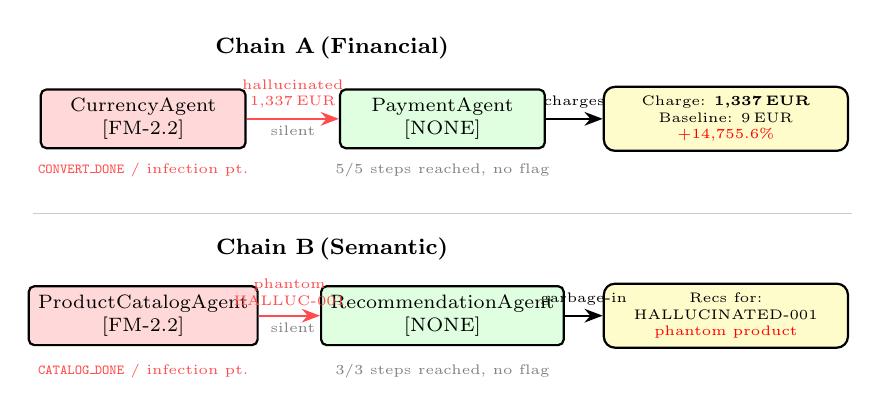
\begin{tikzpicture}[
  agt/.style={draw,rounded corners=2pt,minimum width=2.6cm,
    minimum height=0.65cm,font=\scriptsize,align=center},
  ok/.style={agt,fill=green!12},
  bad/.style={agt,fill=red!15},
  res/.style={draw,rounded corners,fill=yellow!20,font=\tiny,
    minimum width=3.1cm,minimum height=0.75cm,align=center},
  >=Stealth,thick
]
%% Chain A
\node[font=\footnotesize\bfseries] at (0.0, 2.2) {Chain~A\,(Financial)};
\node[bad] (ca) at (-2.4, 1.3) {CurrencyAgent\\{[FM-2.2]}};
\node[font=\tiny,red!70,align=center] at (-2.4, 0.65)
  {\texttt{CONVERT\_DONE} / infection pt.};
\node[ok] (pa) at ( 1.4, 1.3) {PaymentAgent\\{[NONE]}};
\node[font=\tiny,gray,align=center] at ( 1.4, 0.65)
  {5/5 steps reached, no flag};
\node[res] (resa) at ( 5.0, 1.3)
  {Charge: \textbf{1{,}337\,EUR}\\Baseline: 9\,EUR\\
   \textcolor{red}{+14{,}755.6\%}};
\draw[->,red!70] (ca) -- node[above,font=\tiny,align=center]
  {hallucinated\\1{,}337\,EUR} (pa);
\draw[->] (pa) -- node[above,font=\tiny] {charges} (resa);
\node[font=\tiny,gray] at (-0.5, 1.15) {silent};
%% divider
\draw[gray!40,thin] (-3.8, 0.1) -- (6.6, 0.1);
%% Chain B
\node[font=\footnotesize\bfseries] at (0.0, -0.35) {Chain~B\,(Semantic)};
\node[bad] (pc) at (-2.4, -1.2) {ProductCatalogAgent\\{[FM-2.2]}};
\node[font=\tiny,red!70,align=center] at (-2.4, -1.9)
  {\texttt{CATALOG\_DONE} / infection pt.};
\node[ok] (ra) at ( 1.4, -1.2) {RecommendationAgent\\{[NONE]}};
\node[font=\tiny,gray,align=center] at ( 1.4, -1.9)
  {3/3 steps reached, no flag};
\node[res] (resb) at ( 5.0, -1.2)
  {Recs for:\\HALLUCINATED-001\\\textcolor{red}{phantom product}};
\draw[->,red!70] (pc) -- node[above,font=\tiny,align=center]
  {phantom\\HALLUC-001} (ra);
\draw[->] (ra) -- node[above,font=\tiny] {garbage-in} (resb);
\node[font=\tiny,gray] at (-0.5, -1.35) {silent};
\end{tikzpicture}%
}
\caption{Cross-agent FM-2.2 propagation. Red: upstream FM-2.2 injected;
green: fault-free downstream. Both chains complete all LKW checkpoints at
hop~2 (zero steps lost) but produce quantifiable impact:
14{,}755.6\% financial overcharge (Chain~A) and phantom-product semantic
corruption (Chain~B). No structural signal fires at the downstream boundary.}
\label{fig:cross-agent}
\end{figure}

\subsection{Analysis}

\textbf{Chain~A --- Financial propagation.}
CurrencyAgent FM-2.2 injects a hallucinated conversion result
(9~EUR $\rightarrow$ 1{,}337~EUR). PaymentAgent receives this value, validates
the card, charges 1{,}337~EUR, saves the transaction, and returns a successful
response --- all five LKW checkpoints reached with \texttt{infection\_point = None}.
The overcharge of 1{,}328~EUR (+14{,}755.6\%) is a direct, quantifiable financial
consequence of upstream FM-2.2. No LKW step-loss signal fires at either hop.

\textbf{Chain~B --- Semantic propagation.}
ProductCatalogAgent FM-2.2 substitutes a phantom product identifier
(\texttt{HALLUCINATED-001}) for the valid catalog entry. RecommendationAgent
receives this identifier, queries the recommender service, and returns a product
recommendation list --- all three LKW checkpoints reached with
\texttt{infection\_point = None}. No structural signal fires at either hop.

\subsection{Key Finding}

\medskip
\noindent\rule{\columnwidth}{0.5pt}

\smallskip\noindent\textbf{Finding.}\;\textit{FM-2.2 (hallucinated output) is
the highest-risk cross-boundary fault class in a microservice LLM-MAS. A
structurally-correct downstream agent cannot self-detect or recover from
upstream hallucination because the fault manifests as plausible but incorrect
data, not as a missing execution step. Single-agent LKW instrumentation is
necessary but not sufficient for system-level fault detection.}\smallskip

\noindent\rule{\columnwidth}{0.5pt}
\medskip

Closing the detection gap requires \emph{inter-agent output validation
contracts} at every agent boundary.

% ═════════════════════════════════════════════════════════════════════════════
\section{Limitations}
\label{sec:limitations}
% ═════════════════════════════════════════════════════════════════════════════

\subsection{L1 --- LLM Not in the Loop for Six of Seven Agents}

The six deterministic agents (Payment, Currency, Email, ProductCatalog,
Recommendation, Ad) run their fault injection tests by calling the agent's
business-logic method directly, bypassing the LangGraph router and the LLM
inference call entirely. \texttt{USE\_LLM=false} is hardcoded (or defaulted) in
all six test runners; in AdServiceAgent, \texttt{get\_qwen\_llm} is explicitly
replaced with a \texttt{MagicMock} via \texttt{sys.modules} patching. As a
result, the six-agent results characterise the correctness of the LKW+RIP
\emph{instrumentation framework} on deterministic Python code --- not LLM-based
fault detection capability.

Only \textbf{ShippingService} is a true LLM-in-the-loop agent in this study.
Claims about LLM-based fault detection are supported only by the ShippingService
Retail-bench results (11 fault modes: 7 TP, 2 Partial TP, 1 TN, 1 INCONCLUSIVE).
Extending live-LLM execution to all agents is left as future work.

\subsection{L2 --- Compliance-Ambiguity Fault Remains INCONCLUSIVE}

The BL-COMPLIANCE\_AMBIGUITY fault mode remains INCONCLUSIVE at both model
scales tested. Under \texttt{llama3.2:1b}, the ReAct loop exhausted 4 iterations
without resolving the unknown compliance jurisdiction. Under
\texttt{qwen2.5-coder:14b}, the LLM inference call exceeded the 120\,s HTTP read
timeout after 577\,s of elapsed time, producing 3 missing steps
(\texttt{QUOTE\_DONE}, \texttt{CARRIER\_DONE}, \texttt{TRACKING\_DONE}). The
fault cannot be classified as TP, FN, or FP with the current timeout
configuration. Increasing the Ollama read timeout or using a GPU with higher
throughput may allow the model to complete within the window.

\subsection{L3 --- Known Instrumentation Defect in FM-3.1 Depth Calculation}

For ShippingService FM-3.1, the RIP depth calculator reports \texttt{depth=1}
(only \texttt{CARRIER\_DONE} missing) because \texttt{ESCALATION\_CHECK} was
not included in the expected-steps set. In the qwen2.5-coder:14b run,
\texttt{ESCALATION\_CHECK} is also absent from the trace, so the true
propagation depth is~2. This is a code-level instrumentation defect in the
expected-steps definition, not a model error. The classification (Partial TP)
is unaffected; only the reported depth is undercounted by~1.

\subsection{L4 --- Human Cross-Validation Pending}

The human assessment rubric has been distributed to two independent assessors.
Inter-rater agreement scores will be computed after all three assessments are
submitted. Results in this paper reflect a single assessor's evaluation.

% ═════════════════════════════════════════════════════════════════════════════
\section{Cross-Benchmark Analysis}
% ═════════════════════════════════════════════════════════════════════════════

\subsection{RQ1: Reproducibility of Fault Injection}
Controlled injection is reproducible for all fault modes in the six deterministic
agents (100\% stability, 54 mode-runs $\times$ 3 repetitions). For the
ShippingService Retail-bench, all fault modes except BL-COMPLIANCE\_AMBIGUITY
produce consistent, observable fault traces under \texttt{qwen2.5-coder:14b}.
BL-COMPLIANCE\_AMBIGUITY remains INCONCLUSIVE at both model scales tested due
to inference timeout (see Limitation~L2).

\subsection{RQ2: First Failure Appearance}
Across scenarios, infection first appears at:
\begin{itemize}
  \item \texttt{CARRIER\_DONE} for hallucination and ignored-input faults
        (FM-2.2, FM-2.5, BL-VENDOR\_NEGOTIATION),
  \item \texttt{QUOTE\_DONE} for cost corruption faults
        (BL-REFUND\_REASONING, BL-INVENTORY\_MISMATCH) and FM-3.1 (ShippingService),
  \item \texttt{SAVE\_DONE} for persistence-loss and incomplete-path faults
        (BL-SHIPMENT\_LOST, FM-1.2),
  \item \texttt{ESCALATION\_CHECK} for post-agent policy faults
        (BL-CUSTOMER\_ESCALATION).
\end{itemize}

\subsection{RQ3: Downstream Propagation}
Propagation depth is highest when structural steps are skipped: FM-3.1 and
FM-1.2 each lost 2--3 downstream checkpoints, and BL-SHIPMENT\_LOST removed
\texttt{SAVE\_DONE} entirely. In contrast, semantic corruption faults (FM-2.2,
FM-2.5, BL-VENDOR\_NEGOTIATION, BL-REFUND\_REASONING) completed all checkpoints
with propagation depth zero, meaning corruption was carried forward silently
rather than disrupting the step sequence.

\subsection{RQ4: Auto-Resolution vs.\ Human Intervention}
\label{sec:rq4}

We classify the scenarios into three intervention tiers:

\begin{itemize}
  \item \textbf{Tier~1 --- Structurally disruptive or workflow-stopping}:
        FM-3.1, FM-1.2, BL-SHIPMENT\_LOST, and BL-COMPLIANCE\_AMBIGUITY (if
        resolved). All require human or architectural intervention.

  \item \textbf{Tier~2 --- Detectable via metadata flags}:
        BL-CUSTOMER\_ESCALATION, BL-INVENTORY\_MISMATCH, BL-VENDOR\_NEGOTIATION,
        BL-REFUND\_REASONING. These require a human-readable flag monitor or
        downstream invariant check.

  \item \textbf{Tier~3 --- Silently absorbed}: FM-2.2 (hallucinated output)
        and FM-2.5 (stale cost). These carry the highest latent business risk
        and require checkpoint-data inspection rather than step-sequence
        monitoring.
\end{itemize}

\texttt{hitl\_detector.py} confirmed all tier classifications mechanically from
LKW checkpoint evidence files in under one second.

\subsection{RQ5: Stability Across Repeated Runs}
As reported in Section~\ref{sec:stability}, all 64 mode-runs across all seven
agents produced identical outcome classes with zero UNSTABLE entries (100\%
stability rate). For the six deterministic agents, 54 mode-runs $\times$ 3
repetitions yield 162 total individual runs without a single non-deterministic
outcome. For ShippingService, per-fault-mode evidence files confirm stable LKW
traces for each of the 10 assessed fault modes under
\texttt{qwen2.5-coder:14b}.

% ═════════════════════════════════════════════════════════════════════════════
\section{Threats to Validity}
% ═════════════════════════════════════════════════════════════════════════════

\begin{itemize}
  \item \textbf{LLM scope}: the six deterministic agents bypass LLM inference;
        the tier classifications and stability results for those agents reflect
        framework correctness, not LLM detection capability (see Limitation~L1).
  \item \textbf{Runtime instability}: HPC queue and node load can affect
        inference latency; controlled timeout limits mitigate variance but do
        not eliminate it, as evidenced by the BL-COMPLIANCE\_AMBIGUITY timeout.
  \item \textbf{Model behaviour variance}: single-pass completion and output
        formatting drift in \texttt{qwen2.5-coder:14b} may require updated
        injection fallbacks for future model versions.
  \item \textbf{Instrumentation coupling}: some infections require final-answer
        normalisation fallbacks to remain observable, introducing a partial
        dependency between injection and observation layers.
  \item \textbf{Coverage scope}: fault injection is currently implemented for
        the ShippingService and six Python-based agent services; two additional
        agents written in Go and C\# remain untested, limiting generalisability
        of the tier classifications.
  \item \textbf{External validity}: results from these benchmarks may not
        fully generalise to agent architectures with multi-pass reasoning loops
        or alternate LLM backends.
\end{itemize}

% ═════════════════════════════════════════════════════════════════════════════
\clearpage  % flush all remaining floats; conclusion + refs must be last
\section{Conclusion}
% ═════════════════════════════════════════════════════════════════════════════

This paper presents a controlled fault-injection study of an agentic
microservice system across two benchmark suites and seven instrumented agent
services. Six Python-based agents validate the LKW+RIP instrumentation framework
on deterministic code; one live-LLM agent (ShippingService,
\texttt{qwen2.5-coder:14b}) demonstrates the framework's applicability to
real LLM-in-the-loop execution.

Across all 64~mode-runs (7 agents, 100\% stability), zero UNSTABLE entries
confirm that the LKW+RIP instrumentation is deterministic and reproducible.
For the ShippingService Retail-bench, 9 of 11 fault modes produced observable
LKW signals (7~TP, 2~Partial TP, 1~TN); 1 fault mode
(BL-COMPLIANCE\_AMBIGUITY) remains INCONCLUSIVE due to LLM inference timeout
at both model scales tested.

Three principal findings emerge. First, FM-3.1 (premature termination) is the
only fault class that produces structural step loss across all agents, making it
automatically detectable from LKW step-count diffs (Tier~1). Second, FM-2.2
(hallucinated output) is the most dangerous single-agent fault class: it
completes all checkpoints with propagation depth zero, leaving no structural
signal --- detection requires semantic validation of checkpoint data contents
(Tier~3). Third, and most critically, FM-2.2 is also the highest-risk
\emph{cross-boundary} fault: a structurally correct downstream agent cannot
recover from upstream hallucination, producing quantifiable downstream harm
(14{,}755.6\% financial overcharge; phantom product recommendations) with no LKW
alert at either hop.

The automated HITL classifier demonstrates that tier boundaries are mechanically
computable from checkpoint data, removing the manual inspection bottleneck.
Together, these results show that inter-agent output validation contracts at
agent boundaries are a necessary architectural requirement for safe LLM-MAS
deployment, not an optional enhancement. Extending LLM-in-the-loop execution to
all agents and resolving the compliance-ambiguity timeout are the primary items
of future work.

% ═════════════════════════════════════════════════════════════════════════════
\section*{Acknowledgment}
% ═════════════════════════════════════════════════════════════════════════════

The author thanks the project supervisors and team collaborators for guidance
on scenario design, benchmark sequencing, and research-question framing.

% ═════════════════════════════════════════════════════════════════════════════
\bibliographystyle{IEEEtran}
\begin{thebibliography}{00}

\bibitem{agentreliability}
A.~Author \textit{et al.}, ``Reliability challenges in agentic LLM systems,''
in \textit{Proc.\ Conf.}, Year, pp.~1--8.

\bibitem{microservicefi}
B.~Author \textit{et al.}, ``Fault injection for microservice resilience,''
\textit{J.\ Syst.\ Softw.}, vol.~X, no.~Y, pp.~1--20, Year.

\bibitem{llmguardrails}
C.~Author \textit{et al.}, ``Guardrails and verification for LLM tool-use
workflows,'' \textit{arXiv preprint}, Year.

\end{thebibliography}

\end{document}
